\chapter{Lösungsstrategie}

\subsection{Controller}
Der Controller fungiert als Observer. 
Er empfängt Benachrichtigungen vom Modell, wenn Änderungen oder Aktualisierungen erfolgen, und leitet diese Informationen an die View weiter, um sie zu aktualisieren. 
Der Controller speichert keine Zustände und sendet keine Eingaben von der View an das Modell.

%Eventuell später parametertype hinzufügen und genauer definieren.
\begin{table}[h!]
    \centering
    \begin{tabular}{|p{5cm}|p{5cm}|p{5cm}|}
        \hline
        \textbf{Funktion} & \textbf{Voraussetzung} & \textbf{Semantik} \\
        \hline
       void update() & Modell hat Änderungen & Benachrichtigt den Controller, der die View aktualisiert. \\
        \hline
        void updateView(AvailableRobots: String[], SelectedRobotIdx: int, Error: bool, Confirmation: bool) & Gültige Modell-Daten vorhanden & Aktualisiert die View mit den neuesten Daten und Fehlerstatus. \\
        \hline
        void init() & Controller mit Modell verbunden & Registriert den Controller als Observer. \\
        \hline
    \end{tabular}
    \caption{Funktionen des Controllers}
    \label{tab:Controller}
\end{table}

\clearpage
\subsection{Modell}
\begin{table}[h!]
    \centering
    \begin{tabular}{|p{5cm}|p{5cm}|p{5cm}|}
        \hline
        \textbf{Funktion} & \textbf{Voraussetzung} & \textbf{Semantik} \\
        \hline
        ActuatorControlWrapper(Host: String, Port: int, Actuator: String) & Gültige Netzwerkverbindung; Aktuator A1–A4 & Initialisiert Roboterarm mit Host, Port und Aktuator. \\
        \hline
        increase() & Aktuator gesetzt; Verbindung besteht & Erhöht den Steuerwert um 1 und ruft applyValue() auf. \\
        \hline
        decrease() & Aktuator gesetzt; Verbindung besteht & Verringert den Steuerwert um 1 und ruft applyValue() auf. \\
        \hline
        applyValue() & Aktuator gültig; Wert im Bereich [0,100] & Wendet den aktuellen Wert auf den Aktuator an. \\
        \hline
        addListener() & Listener gültig & Fügt einen Listener hinzu, der bei Zustandsänderung benachrichtigt wird. \\
        \hline
        removeListener() & Listener gültig & Entfernt den angegebenen Listener. \\
        \hline
        setSelectedRobot(String) & Roboter in availableRobots & Setzt den aktuellen Roboter und benachrichtigt alle Listener. \\
        \hline
        getSelectedRobot() & Objekt initialisiert & Gibt den aktuell ausgewählten Roboter zurück. \\
        \hline
        getActuator() & Objekt initialisiert & Gibt den aktuellen Aktuator zurück. \\
        \hline
        getValue() & Objekt initialisiert & Gibt den aktuellen Steuerwert zurück. \\
        \hline
        addAvailableRobot(String) & Gültige Roboter-ID & Fügt einen Roboter zur Liste verfügbarer Roboter hinzu. \\
        \hline
        removeAvailableRobot(String) & Gültige Roboter-ID & Entfernt einen Roboter aus der Liste verfügbarer Roboter. \\
        \hline
        getAvailableRobots() & Keine & Gibt alle bekannten Roboter zurück. \\
        \hline
    \end{tabular}
    \caption{Funktionen des Modells}
    \label{tab:Methodenbeschreibung}
\end{table}

\clearpage
\subsection{View}
Die View besteht aus den unabhängigen Blöcken IO und UI. Die UI bietet eine Softwareschnittstelle an, die IO keine.

\subsubsection{IO Funktionen}
\begin{table}[h!]
    \centering
    \begin{tabular}{|p{5cm}|p{5cm}|p{5cm}|}
        \hline
        \textbf{Funktion} & \textbf{Voraussetzung} & \textbf{Semantik} \\
        \hline
        void readInputs() & Eingabe durch den Benutzer erfolgt & Überprüft die Benutzereingaben und löst entsprechende Aktionen aus. \\
        \hline
        int initIO() & IO-Hardware verfügbar & Initialisiert und überprüft die IO-Hardwareschnittstellen und gibt einen Fehlercode bei Problemen zurück. \\
        \hline
    \end{tabular}
    \caption{IO Funktionen}
    \label{tab:IOFunktionen}
\end{table}

\subsubsection{UI Funktionen}
\begin{table}[h!]
    \centering
    \begin{tabular}{|p{5cm}|p{5cm}|p{5cm}|}
        \hline
        \textbf{Funktion} & \textbf{Voraussetzung} & \textbf{Semantik} \\
        \hline
        void updateView(AvailableRobots: String[],SelectedRobotIdx: int, Error: bool, Confirmation: bool) & Gültige Modell-Daten vorhanden & View-Schnittstelle. Aktualisiert die UI mit den neuesten Roboter-Daten und Statusinformationen (Fehler, Bestätigung). \\ 
        \hline
    \end{tabular}
    \caption{UI Funktionen}
    \label{tab:UIFunktionen}
\end{table}

\begin{figure}[h]
  \centering
  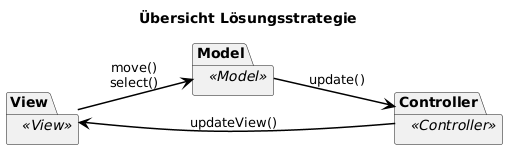
\includegraphics[width=0.5\textwidth]{diagrams/Übersicht_Lösungsstrategie.png}
  \caption{Übersicht Lösungsstrategie}
  \label{fig:baustein}
\end{figure}







%\subsection*{Grafische Darstellung}

%Ein Qualitätsziel ist die Intuitive Benutzbarkeit der Software. Dies ausschließlich mit Lichtern und Knöpfen darzustellen scheint unrealistisch. Folgende Funktionalität wird unsere Grafische darstellung benötigen:
%
%**Schnittstelle (Interface):**
%
%\begin{Java}[caption={Utility Types}]
%class Position {
%	int rotation;   // Values in range [0-100]
%	int joint1;     // Values in range [0-100]
%	int joint2;     // Values in range [0-100]
%	int claw;       // Values in range [0-100]
%}
%
%class RobotArm {
%	String name;    // Identifier to display to user
%	int id;         // Actual identifier 
%}
%
%enum Movement {
%	// Rotation
%	ROTATE_CLOCKWISE,
%	ROTATE_COUNTERCLOCKWISE,
%	// First Joint
%	JOINT1_OPEN,
%	JOINT1_CLOSE,
%	// Second Joint
%	JOINT2_OPEN,
%	JOINT2_CLOSE,
%	//Claw
%	CLAW_OPEN,
%	CLAW_CLOSE
%}
%%\end{Java}
%%
%\newpage
%
%\begin{Java}[caption={Interfaces}]
%// UI is about user feedback
%interface UI {
%	void displaySelectOptions(RobotArm[] robotArms);
%    // Update display of selected Robot
%	void displaySelected(RobotArm robotArm);
%    // Update display of arm status
%	void displayArmStatus(Position position);
%    // Update display of error message
%	void displayError(String message);
%}
%
%// IO is about user input
%interface IO {
%    // Callback signature: void callback(Movement movement) 
%	void onMoveCommand(Function<Movement> callback);
%	// Callback signature: void callback(RobotArm robotArm) 
%    void onSelect(Function<RobotArm> callback);
%}
%
%// ActuatorController is about Interacting with the Robot
%// Wrapper for ICaDSRoboticArm
%interface ActuatorController {
%    /**
%     * Moves the actuator incrementally.
%     * 
%     * This method performs an incremental movement for the actuator 
%    * and returns the duration of the movement in milliseconds. If the 
%     * robot cannot be reached, a {@link CouldNotReachRobotException}  
%     * is thrown to indicate the failure.
%     * @return the duration of the movement in milliseconds
%     * @throws CouldNotReachRobotException if the robot cannot be 
%     *      reached or moved (e.g., due to connectivity issues or 
%     *      other reasons)
%     */
%    int move(Movement movement) throws CouldNotReachRobotException;
%    /**
%     * Gets the current position of the actuators.
%     * 
%     * If the robot cannot be reached, a 
%     * {@link CouldNotReachRobotException} is thrown to indicate the 
%     * failure.
%    * @return the current position of the actuators.
%     * @throws CouldNotReachRobotException if the robot cannot be 
%     *      reached or moved (e.g., due to connectivity issues or 
%     *      other reasons)
%     */
%    Position getPosition() throws CouldNotReachRobotException;
%}
%\end{Java}
%--------------------------------Comments--------------------------------
% // ICaDSRoboticArm is the given interface
% interface ICaDSRoboticArm {
% 	// Is in Range: [0 - 100] Forth := 100 Back := 0
% 	int getBackForthPercentage();
% 	// Is in Range: [0 - 100] Left := 100 Right := 0
% 	int getLeftRightPercentage();
% 	// Open := 100 Close := 0 Is in Range: [0 - 100]
% 	int getOpenClosePercentage();
% 	// Is in Range: [0 - 100] Up := 100 Down := 0
% 	int getUpDownPercentage();
% 	// Real: returnValue := true if the robotic arm is active and communicating, false if not 
% 	// Simulation: returnValue := always true
% 	boolean heartbeat();
% 	// initializations for the robot
% 	boolean init();
% 	// Set Target Percentage Only percentages in the specified range are supported.
% 	void setBackForthPercentageTo(int percentage);
% 	// Set Target Percentage Only percentages in the specified range are supported.
% 	void setLeftRightPercentageTo(int percentage);
% 	// Set Target Percentage Only percentages in the specified range are supported.
% 	void setOpenClosePercentageTo(int percentage);
% 	// Set Target Percentage Only percentages in the specified range are supported.
% 	void setUpDownPercentageTo(int percentage);
% 	// shutdown robotic arm
% 	void teardown();
% 	// wait till init-process is finished
% 	void waitUntilInitIsFinished();
% }	
% '''ts
% interface GUI {
%     displayArmStatus(status: ArmStatus): void
%     onMoveCommand(callback: (command: MoveCommand) => void): void
%     onGripCommand(callback: (grip: boolean) => void): void
%     showError(message: string): void
% }

% type MoveCommand = {
%     x: number       // Position in X-Richtung
%     y: number       // Position in Y-Richtung
%     z: number       // Position in Z-Richtung
% }

% type ArmStatus = {
%     position: MoveCommand   // aktuelle Position des Arms
%     gripperOpen: boolean    // Zustand des Greifers (offen/geschlossen)
%     error?: string          // optionaler Fehlertext
% }
% '''

% TODO: Architekturdiagramm zur Schichtenstruktur und Kommunikationsbeziehungen einfügen

% Grundlage ist ein bi-direktionales Client-Server-Modell, das auf die Anforderungen ( KAPITEL)
% %TODO Kapitel
% zugeschnitten ist.
 

% \begin{itemize}
% 	\item{Client:} Dieser besteht aus einer GUI-Software auf dem ITS-Board, das über ein integriertes Display eine grafische Benutzeroberfläche (GUI) zur Verfügung stellt. Die Interaktion erfolgt über Buttons, die Steuerbefehle auslösen. Das ITS-Board kommuniziert mit der Roboter-Software, die auf dem Raspberry Pi des zu steuernden Roboterarms, liegt.
	
% 	\item{Server:} Die Roboter-Software liegt auf dem Raspberry Pi der Roboterarme. Sie verwaltet den Verbindungszustand, koordiniert die einkommenden Steuerbefehle und leitet/übersetzt Anfragen gezielt an den Roboterarm weiter. Zusätzlich sendet sie als einen Heartbeat an die GUI-Software. Die Roboter-Software führt einen Registrierung durch mit einem eindeutigen Bezeichner (Name oder ID) , und einem status beim ITS-Board durch
% 	Der Server umfasst auch die Roboter selbst sowie deren lokale Steuereinheit und Sensorik. Jeder Roboter betreibt eine eigene API zur Steuerung und stellt Statusinformationen bereit. 	
% \end{itemize} 

% Die Kommunikation zwischen dem Client und Servern erfolgt über TCP/IP. Die Wahl von TCP garantiert eine zuverlässige, geordnete und fehlerfreie Datenübertragung. Um jedoch Verbindungsabbrüche rechtzeitig zu erkennen, wird zusätzlich ein Heartbeat-Mechanismus (Watchdog) auf in der GUI-Software eingesetzt, der regelmäßig geprüft wird (siehe Metriken, Kapitel 
% %TODO hier richtigen verweis einfügen
% ). Jede Roboter-Software muss sich nach dem Systemstart aktiv bei dem ITS-Board registrieren. Die GUI-Software verwaltet eine zentrale Teilnehmerliste in Form einer Tabelle mit Tupeln der Form     exttt{(Name, IP-Adresse, Status)}. Diese wird zur Adressierung und gezielten Kommunikation verwendet. % TODO Wie genau muss das dann passieren Stichwort asynchron usw...
% \\\\
% In der GUI werden nur die erreichbaren Roboterarme aufgeführt. So kann sich der Benutzer einen der Roboterarme aussuchen zu diesem eine TCP Verbindung aufbauen und diesen anschließend per Buttons steuern. Durch den Abbruch der vorherigen Verbindung werden evtl. vorherige bewegte Roboterarme gestoppt. Dadurch ist gesichert, dass immer nur ein Roboterarm gesteuert wird. Sollte ein Roboterarm ausfallen bzw. vom Netz getrennt werden, ist dieser Roboterarm mit dem status "offline" gekennzeichnet. Alle Bewegungen dieses Roboters werden sofort beendet. Ebenfalls wird die GUI-Software mit einem Not-Aus über einen Button ausgestattet, sodass der ausgewählte Roboter sofort jede Bewegung abbricht. Die Ansteuerung des Roboters erfolgt mit dem RPC-Protokoll. Dadurch wird regelmässig eine Funktion auf der Roboter-Software aufgerufen, anschliessend übersetzt und die Bewegung am Roboterarm durchgeführt. Das Statusupdate des jeweiligen Roboterarms kann dann per RPC von der Roboter-Software zum ITS-Board erfolgen.


% \subsection*{Überprüfung der Lösungsstrategie}
% %TODO Überarbeiten und überprüfen
% \subsubsection*{Ziele für Software Engineering}

% \begin{itemize}
% 	\item     extbf{Client-Server}: Es existiert genau ein Client und mehrere Server, die einzeln angesprochen werden können. Die Server haben alle die gleiche API und Funktionaliät (SE-Ziele Funktionalität, Skalierbarkeit, Wartbarkeit, Anpassbarkeit, Kompatibilität)
% 	\item     extbf{Watchdog}: Roboter-Software und Roboter überwachen gegenseitig den Verbindungsstatus, um bei Abbruch in einen sicheren Zustand zu wechseln. (SE-Ziel Safety)
% 	\item     extbf{Kommunikationsprotokoll:} TCP/IP wurde gewählt, um eine zuverlässige, verbindungsorientierte Kommunikation zu gewährleisten. RPC wurde gewählt, da so eine funktionale Umsetzung konsequent durchgeführt wird.
% 	\item     extbf{Adressierung:} Die Teilnehmer befinden sich im selben /24-Netzwerk und kommunizieren über IPv4. Jeder Roboter benötigt eine eindeutige ID oder Namen.
% \end{itemize}

% \subsection*{Ziele für Verteilte Systeme}
% \begin{itemize}
% 	\item     extbf{Ressourcenteilung:} Alle Roboter können einheitlich über eine GUI-Software des ITS-Boards gemeinsam verwendet werden.
% 	\item     extbf{Offenheit:} Neue Roboter können sich dynamisch am ITS-Board registrieren. Das System bleibt erweiterbar ohne strukturelle Änderungen.
% 	\item     extbf{Skalierbarkeit:} Das Netzwerk begrenzt die Anzahl der Roboterarme. Diese registrieren sich mit aktualisierenden Status bei der GUI-Software des Clients
% 	\item     extbf{Verteilungstransparenzen:} Durch das Client-Server Modell und das MMI über die GUI werden die Verteilungstransparenzen teilweise eingehalten. Die Architektur versteckt die konkrete Lage und Ansteuerung der Roboter (Ortstransparenz, Zugriffstransparenz) vor dem Nutzer. Die GUI zeigt nur logische Namen an, nicht IP-Adressen oder spezifische Schnittstellen.
% \end{itemize}


% \subsection*{Schwächen}
% \begin{itemize}
% 	\item Netzwerk kann durch UDP-Anfragen "lahmgelegt werden", Watchdog an Roboter-Software und am Roboterarm darf also nicht auf Antwort warten
% 	\item Ziel Leistung: Leistung des Systems durch ITS-Board Hardware abhängig. (Befehle pro Sekunde). Das ITS-Board ist aber sehr eingeschränkt in Speicher und Leistungsfähigkeit.
% 	\item Fehlertransparenz: GUI zeigt nicht verfügbaren Roboter nicht mehr an.
% 	\item Skalierbarkeitstransparenz: Neue Roboter könnten durch zu Leistungseinbrüchen des Systems durch ITS-Board führen
% 	\item Lokalitätstransparenz: Ist durch den eindeutigen Namen nicht gegeben und durch Hinzufügen bzw. Verschwinden auf der GUI nicht gegeben.
% \end{itemize}


%     extbf{Alternative Überlegung:}

% Um das ITS-Board zu entlasten.

% \begin{itemize}
% 	\item Die Roboter melden sich bei einem Service an und diese verwaltet und überprüft die Verfügbarkeit der Roboter und des ITS-Boards. Die Liste der verfügbaren Roboter wird dem ITS-Board übermittelt. Dieser Service läuft auf der ICC Cloud, dafür wird auf einem Rechner im Netzwerk ein Proxy eingerichtet, der die Anfragen weiterleitet.
% 	\begin{itemize}
% 		\item Vorteil: Rechenlast ausgelagert
% 		\item Nachteil: Single Point of Failure durch Proxy
% 	\end{itemize}
% 	\item Die Raspberry Pi tauschen sich untereinander aus, wer die Liste an das ITS-Board sendet. So ist das Gesamtsystem ausfallsicher. Die Raspberry Pi wissen alle voneinander.
% 	\begin{itemize}
% 		\item Vorteil: Kein Single Point of Failure, Rechenlast auf Rapberry Pi, der schon im System vorhanden ist und somit keine neue Fehlerquelle.
% 		\item Nachteil: Erhöhter Verwaltungsaufwand
% 	\end{itemize}
% \end{itemize}





